\documentclass[../main.tex]{subfiles}
\begin{document}
\chapter{Real Numbers}
\section{Constructions using \texorpdfstring{$\N$}{the naturals}}
Recall the construction of $\N$ using the Peano axioms from \cref{naturalDef}.
We can build on this construction to formally define the \textit{integer} and \textit{rational} numbers.
\subsection{Integers\texorpdfstring{ -- $\Z$}{}}
We obtain $\Z$ from $\N$ by allowing for subtraction, formally, $\Z$ is the equivalence classes of $\N \times \N$ under the equivalence relation:
\[
  (a, b) \rel (c, d) \iff a + d = b + c
\]
That is, $\Z$ is the quotient $\Z = (\N \times \N) / R$.
Think of $(a, b)$ as representing the operation $a - b$.
We write $0$ for $[(1, 1)]$ and $-a$ for $[(1, 1 + a)]$.
We also define addition and multiplication operations by:
\begin{align*}
  (a, b) + (c, d) &= (a + c, b + d) \\
  (a, b) \times (c, d) &= (ac + bd, bc + ad)
\end{align*}
which satisfy the usual rules of arithmetic.

\subsection{Rationals\texorpdfstring{ -- $\Q$}{}}
We obtain $\Q$ from $\Z$ by allowing for division.
Formally, $\Q$ is the set of equivalence classes of $\Z \times \N$ under an equivalence relation:
\[
  (a, b) \rel (c, d) \iff ad = bc
\]
That is, $\Q$ is the quotient $\Q = (\Z \times \N) / R$.
We write $\frac{a}{b}$ for $[(a, b)]$.
We also define additional and multiplication by:
\begin{align*}
  (a, b) + (c, d) &= (ad + bc, bd) \\
  (a, b) \times (c, d) &= (ac, bd)
\end{align*}
which satisfy the usual rules of arithmetic.

We can also define an order on $\Q$, denoted $<$, which has the properties:
\begin{enumerate}
  \item \textbf{Trichotomy -} If $a, b \in \Q$ then exactly one of:
    \[
      a < b \qquad a = b \qquad b < a
    \]
    holds.
  \item \textbf{Transitivity -} If $a < b$ and $b < c$ then $a < c$.
\end{enumerate}
This ordering on $\Q$ has the useful property that between any 2 rational numbers, there is another rational number.
That is, if $p, q \in \Q$ with $p < q$, then $p < \frac{p + q}{2} < q$.
\section{Gaps in the Rationals}
\begin{proposition}
  There is no rational number $x$ with $x^2 = 2$.
\end{proposition}
\begin{proof}[1]
  Suppose $x^2 = 2$.
  Note we may assume that $x > 0$ since $(-x)^2 = x^2$.
  If $x$ is rational, then $x = \frac{a}{b}$ for some $a, b \in \N$.
  Then:
  \[
    \frac{a^2}{b^2} = 2 \iff a^2 = 2b^2
  \]
  But the exponent of 2 in the prime factorisation of $a^2$ is even, while the exponent of 2 in the prime factorisation of $2b^2$ is odd.
  Since prime factorisations are unique by \cref{uniquePrimeFactorisation}, this is a contradiction.
\end{proof}
\begin{remark}[Note]
  The same proof shows that if there exists $x \in \Q$ with $x^2 = n$ for some $n \in \N$, then $n$ must be a square number.
\end{remark}
\begin{proof}[2]\par
  \textbf{Part 1 -}
  Suppose $x^2 = 2$ for some $x = \frac{a}{b}$ with $a, b \in \N$.
  Then, given any $c, d \in \Z$, $cx + d$ is of the form $\frac{e}{b}$ for some $e \in \Z$.
  Thus if $cx + d > 0$, then $cx + d \geq \frac{1}{b}$ as 1 is the smallest positive value for $e$.

  \textbf{Part 2 -}
  Now consider that as $1 < x < 2$, we have $0 < x - 1 < 1$.
  So we can pick a sufficiently large $n \in \N$ such that:
  \[
    0 < (x - 1)^{n} < \frac{1}{b}
  \]
  We can then use the binomial theorem (\cref{binomialTheorem}) to expand $(x - 1)^{n}$.
  After, we can then replace all factors of $x^2$ with 2 to write $(x - 1)^{n}$ in the form $cx + d$ for some $c, d \in \Z$.
  So we then have:
  \[
    0 < cx + d < \frac{1}{b}
  \]
  \textbf{Contradiction -}
  Since we have $cx + d > 0$ for some $c, d \in \Z$ in part 2, we must also have $cx + d \geq \frac{1}{b}$ by part 1.
  But this contradicts the fact that $cx + d < \frac{1}{b}$.
  So there does not exist an $x \in \Q$ such that $x^2 = 2$.
\end{proof}
So $\Q$ has ``gaps'', but how do we express this fact making reference only to $\Q$?
$\Q$ in fact fails another property which is key to constructing the reals.
\begin{example}
  \label{rationalUpperBound}
  Let $A$ be the set of positive rationals $p$ such that $p^2 < 2$.
  That is:
  \[
    A = \{p \in \Q : p^2 < 2\}
  \]
  We can show that $A$ contains no largest element.
  For any $p \in A$, consider $q = p - \frac{p^2 - 2}{p + 2}$.
  Since $p \in A$, $p^2 - 2 < 0$ so $q > p$.
  We can also see that:
  \begin{align*}
    q^2 - 2 &= p^2 - \frac{2p(p^2 - 2)}{p + 2} + \frac{(p^2 - 2)^2}{(p + 2)^2} - 2 \\
            &= \frac{(p^2 - 2)(p + 2)^2 - 2p(p^2 - 2)(p + 2) + (p^2 - 2)^2}{(p + 2)^2} \\
            &= \frac{(p^2 - 2)(p^2 + 4p + 4 - 2p^2 - 4p + p^2 - 2)}{(p + 2)^2} \\
            &= \frac{2(p^2 - 2)}{(p + 2)^2} < 0
  \end{align*}
  So $q^2 < 2$, thus $q \in A$.
  This means for any $p \in A$, we can always construct some $q \in A$ such that $q > p$.
  That is, $A$ has no largest element in $\Q$.

  Similarly the set $\{q \in \Q: q > 0,\ q^2 > 2\}$ contains no smallest element in $\Q$.
\end{example}
Crucially, in $\Q$, there is no \textit{least upper bound}.
This is what we mean when we say $\Q$ has ``gaps''.
\section{Defining Real Numbers}
\begin{definition}[Bounded Above]
  We say that a set $S$ is \textit{bounded above}, if there exists some $x \in \R$ such that $x \geq y$ for all $y \in S$.

  Such an $x$ is called an \textit{upper bound} for $S$.
\end{definition}
\begin{definition}[Least Upper Bound]
  We say that $x$ is a \textit{least upper bound} for $S$ if $x$ is an upper bound for $S$ and every other upper bound $x'$ satisfies $x' \geq x$.
\end{definition}
\begin{remark}[Uniqueness]
  Suppose both $a$ and $b$ are distinct least upper bounds for $S$.

  Since $a$ is a least upper bound and $b$ is another upper bound, $b \geq a$.
  Similarly, $b$ is a least upper bound and $a$ is another upper bound, $a \geq b$.
  But then we have $b \leq a$ and $a \leq b$ so $a = b$ which is a contradiction so the least upper bound is unique.

  So we can say that $x$ is \textit{the} least upper bound.
\end{remark}
\begin{remark}[Notation]
  When $x$ is the upper bound for $S$ we may write:
  \[
    x = \operatorname{supremum} S \text{ or } x = \sup S
  \]
\end{remark}
\begin{definition}[Real Numbers]
  The \textit{real numbers}, denoted $\R$, are a set with elements 0 and 1 ($0 \neq 1$), equipped with addition, multiplication, and an ordering $<$, satisfying the following:
  \begin{enumerate}
    \item Addition is commutative and associative with identity 0, and every $x$ has an inverse under addition.
    \item Multiplication is commutative and associative with identity 1, and every $x \neq 0$ has an inverse under multiplication.
    \item Multiplication is distributive over addition, that is:
      \[
        \forall a, b, c \quad a \times (b + c) = a \times b + a \times c
      \]
    \item For all $a, b$, exactly one of:
      \[
        a < b \quad a = b \quad b < a
      \]
      holds, and for all $a, b, c$:
      \[
        a < b \text{ and } b < c \implies a < c
      \]
    \item For all $a, b, c$:
      \[
        a < b \implies a + c < b + c
      \]
      and, if $c > 0$, then:
      \[
        a < b \implies ac < bc
      \]
    \item Given any set $S$ of real numbers that is non-empty and bounded above, $S$ has a least upper bound.
  \end{enumerate}
\end{definition}
\begin{remark}[Note]
  Axiom \textbf{vi} in the above definition is known as the \textit{least upper bound axiom}.
\end{remark}
\begin{remark}[Note]
  This is the axiomatic definition of the real numbers.
  However, there is also other ways to construct the reals that produces the same result.
\end{remark}
\begin{remark}[Remarks]
  \begin{itemize}
    \item Using axioms \textbf{iv} and \textbf{v}, we can check, for example, that $0 < 1$.
      By axiom \textbf{iv} and the restriction $1 \neq 0$, we must have one of either $1 < 0$ or $1 > 0$.
      Suppose, for contradiction, that $1 < 0$.
      \begin{align*}
        1 &< 0 \\
        1 - 1 &< 0 - 1 \text{ by axiom \textbf{v}} \\
        0 &< - 1 \\
        0 \times (-1) &< (-1) \times (-1) \text{ by axiom \textbf{v} and we have $-1 > 0$} \\
        0 &< 1
      \end{align*}
      which is a contradiction.
      Thus we must have $0 < 1$.

      Indeed, if not, then $1 < 0$ as $0 \neq 1$, so $0 = 1 - 1 < 0 - 1 = -1$ so $0 = 0 \times (-1) < (-1)(-1) = 1$ which contradicts $1 < 0$.
    \item We may consider $\Q$ as contained in $\R$, $\Q \subset \R$, by identifying $\frac{a}{b} \in \Q$ with $a \times b^{-1} \in \R$ where $b^{-1}$ is the multiplicative inverse of $b$.
    \item $\Q$ does not satisfy \textbf{vi} as the set $A$ of positive rationals $x$ such that $x^2 < 2$ does not have a supremum inside $\Q$. See \cref{rationalUpperBound}.
    \item In axiom \textbf{vi}, the words ``non empty'' and ``bounded above'' are crucial.
      If $S$ is empty, then every $x \in \R$ is an upper bound for $S$, so there is no least upper bound.
      If $S$ is not bounded above, then it has no upper bounds so certainly has no least upper bound.
  \end{itemize}
\end{remark}
\begin{example}
  \begin{enumerate}
    \item $S = \{x \in \R: 0 \leq x \leq 1\} = [0, 1]$.
      2 is an upper bound for $S$ as for any $x \in S$, $x \leq 2$.
      The least upper bound for $S$, $\sup S = 1$ because:
      \begin{itemize}
        \item 1 is an upper bound, as for any $x \in S$, $x \leq 1$.
        \item Any other upper bound $y$ is such that $y \geq 1$ as $1 \in S$.
      \end{itemize}
    \item $S = \{x \in \R: 0 < x < 1\} = (0, 1)$.
      2 is an upper bound for $S$ as for any $x \in S$, $x \leq 2$.
      The least upper bound for $S$, $\sup S = 1$ because:
      \begin{itemize}
        \item 1 is an upper bound, as for any $x \in S$, $x \leq 1$.
        \item Suppose there is an upper bound $c$ such that $c < 1$.
          We have $0 < c < 1$ so $\frac{1}{2} < \frac{c + 1}{2} < 1$.
          Thus $\frac{c + 1}{2} \in S$ but $\frac{c + 1}{2} > c$ so $c$ is not an upper bound.
      \end{itemize}
  \end{enumerate}
\end{example}
\begin{remark}[Warning]
  If $S$ has a greatest element, then $\sup S = \max S \in S$.
  But the supremum of a set can exist even when $\max S$ does not, in which case $\sup S \notin S$.
\end{remark}
\begin{proposition}[Axiom of Archimedes]
  \label{axiomArchimedes}
  $\N$ is not bounded above in $\R$.
\end{proposition}
\begin{proof}
  Suppose, on the contrary, that $\N$ is bounded above in $\R$.
  Let $c = \sup \N$.
  By definition, $c - 1$ cannot be an upper bound for $\N$ as it is less than $c$.
  So there is $n \in \N$ such that $n > c - 1$.
  But then $n + 1 \in \N$ with $n + 1 > c$ which contradicts the fact that $c$ was an upper bound for $\N$.
\end{proof}
\begin{corollary}
  \label{archimedesCorollary}
  For any real number $t > 0$, there exits an $n \in \N$ such that $\frac{1}{n} < t$.
\end{corollary}
\begin{proof}
  Given $t > 0$, by the axioms of Archimedes, there exits an $n \in \N$  such that $n > \frac{1}{t}$, hence $\frac{1}{n} < t$.
\end{proof}
\begin{definition}[Bounded Below]
  A set $S$ is said to be \textit{bounded below}, if there exist an $x \in \R$ such that $x \leq y$ for all $y \in S$.
  Such an $x$ is called a \textit{lower bound} for $S$.
\end{definition}
If $S$ is non-empty and bounded below, then
\[
  -S = \{-y: y \in S\}
\]
is non empty and bounded above.
So it must have a least upper bound by axiom \textbf{vi}, say $c$.
Hence $-c$ is a greatest lower bound for $S$.
\begin{remark}[Notation]
  When $x$ is the greatest lower bound for $S$ we may write:
  \[
    x = \operatorname{infimum} S \text{ or } x = \inf S
  \]
\end{remark}
\Cref{archimedesCorollary} immediately implies that:
\[
  \inf\left(\left\{\frac{1}{n}: n \in \N\right\}\right) = 0
\]
Suppose we had an lower bound $t > 0$, then there exists an $n \in \N$ such that $\frac{1}{n} < t$ so $t$ is not a lower bound.
So 0 is the infimum.

The previous proposition and corollary show that there are no ``infinitely large'' or ``infinitely small'' numbers in $\R$.

\begin{example}
  Let $S=\{0, \frac{1}{2}, \frac{2}{3}, \frac{3}{4}, \ldots\} = \{1 - \frac{1}{n}: n \in \N\}$.
  Clearly 1 is an upper bound for this set.

  Suppose we have some $c < 1$ is an upper bound for $S$.
  Then $1 - \frac{1}{n} \leq c\ \forall n \in \N$ so $0 < 1 - c \leq \frac{1}{n}\ \forall n \in n$ which contradicts \cref{archimedesCorollary}.
  So $\sup S = 1$.
\end{example}
\begin{theorem}
  There exists $x \in \R$ with $x^2 = 2$.
\end{theorem}
\begin{proof}
  Let $S = \{ x \in \R: x^2 <2\}$.
  Note that $S$ is nonempty since $1 \in S$.
  It is also bounded above, for example, by 2.
  Hence it has a supremum, $c = \sup S$.
  Observe that $1 < c < 2$.
  We claim that $c^2 = 2$.

  Suppose that $c^2 < 2$.
  For $0 < t < 1$, we have:
  \begin{align*}
    (c + t)^2 &= c^2 + 2ct + t^2 \\
              &< c^2 + 4t + t \\
              &= c^2 + 5t \\
              &< 2 \text{ for sufficiently small $t$, e.g. $t < \frac{2 - c^2}{5}$}
  \end{align*}
  This contradicts the fact that $c$ is an upper bound for $S$ since $c + t \in S$ and $c + t > c$.

  Suppose that $c^2 > 2$.
  For $0 < t < 1$, we have:
  \begin{align*}
    (c - t)^2 &= c^2 - 2ct + t^2 \\
              &> c^2 - 4t + 0 \\
              &> 2 \text{ for sufficiently small $t$, e.g. $t < \frac{c^2 - 2}{4}$}
  \end{align*}
  This contradicts the fact that $c$ is a least upper bound for $S$ since $c - t < c$ and $(c - t)^2 > 2$ so $c - t$ is an upper bound for $S$.

  Therefore, by trichotomy, $c^2 = 2$.
\end{proof}
\begin{remark}
  The same proof shows that $\sqrt[n]{x}$ for all $n \in \N, x \in \R, x > 0$.
  That is:
  \[
    \forall n \in \N,\ \forall x \in \R, x > 0\ \exists y \in \R \text{ s.t. } y^n = x
  \]
\end{remark}
\begin{definition}[Irrational]
  A real number that is not rational is called \textit{irrational}.
\end{definition}
\begin{example}
  $\sqrt{2}, \sqrt{3}, \sqrt{6}, \ldots$ are irrational.
  Also $2 + 3\sqrt{5}$ is irrational as suppose we had $2  + 3 \sqrt{5} = \frac{a}{b}$ with $a, b \in \N$, then $\sqrt{5} = \frac{a - 2b}{3b} \in \Q$ which is a contradiction.
\end{example}
\begin{proposition}
The rationals are \textit{dense} in the reals.

This means that if we take any 2 real numbers $a < b \in \R$, there exists a $c \in \Q$ with $a < c < b$.
\end{proposition}
\begin{proof}
  WLOG, assume $a \geq 0$.
  By \cref{archimedesCorollary}, there exists an $n \in \N$ with $\frac{1}{n} < b - a$.
  Let
  \[
    T = \left\{k \in \N: \frac{k}{n} \geq b\right\}
  \]
  By \cref{axiomArchimedes}, there exists $N \in \N$ such that $N > b$.
  Since $N > b$, $Nn \in T$, so $T \neq \emptyset$.
  Therefore, by the Well-Ordering Principle (\cref{WOP}), $T$ has a least element $m$.
  Set $c = \frac{m - 1}{n}$.
  $m$ is the least element of $T$ so $m - 1 \notin T$, that is, $\frac{m - 1}{n} < b$ so $c < b$.

  Now suppose that $c \leq a$.
  Then $\frac{m}{n} = c + \frac{1}{n} < a + (b - a) = b$, which contradicts the fact that $m$ is the least element of $T$.
  Therefore $c > a$.

  So we have constructed $c \in \Q$ such that $a < c < b$.
\end{proof}
\begin{corollary}
  The irrationals are \textit{dense} in the reals.

  That is, for all $a < b \in \R$, there exists a $c \in \R \setminus \Q$ with $a < c < b$.
\end{corollary}
\begin{proof}
  From the above, take a $c \in \Q$ such that $a\sqrt{2} < c < b\sqrt{2}$.
  We then have $a < \frac{c}{\sqrt{2}} < b$.
  $\frac{c}{\sqrt{2}}$ is irrational so we are done.
\end{proof}
\section{Sequences}
\begin{definition}[Sequence]
  A \textit{sequence} is an enumerated collection of objects in which repetitions are allowed and order matters.

  We write $a_1, a_2, \ldots$ or $(a_n)^{\infty}_{n=1}$.
\end{definition}
What does it mean for a sequence $a_1, a_2, \ldots$ to tend to a limit $\ell$?

It is \textbf{not} enough that the terms get closer to $\ell$.
For example, we would not want $0, \frac{1}{2}, \frac{2}{3}, \frac{3}{4}, \ldots$ to tend to 35 as technically each term gets closer to 35.

It is also \textbf{not} enough just that the terms get ``arbitrarily'' close to $\ell$, in the sense that
\[
  \forall \varepsilon > 0, \exists n \in \N \text{ s.t. } \ell -\varepsilon < a_n < \ell + \varepsilon
\]
For example, $0, 10, \frac{1}{2}, 10, \frac{2}{3}, 10, \frac{3}{4}, 10, \frac{4}{5}, 10, \ldots$ satisfies the above but we would not want this to tend to 1.

We want the sequence to both get and stay within $\varepsilon$ of $\ell$.
\subsection{Convergence and Divergence}
\begin{definition}[Convergence]
  \label{convergenceDef}
  We say that the sequence $a_1, a_2, \ldots$ \textit{tends} or \textit{converges} to the limit $\ell \in \R$ as $n$ tends to infinity if:
  \[
    \forall\varepsilon > 0, \exists N \in \N \text{ s.t. } \forall n \geq N, \ell - \varepsilon < a_n < \ell +\varepsilon
  \]
  or more compactly:
  \[
    \forall \varepsilon > 0, \exists N \in \N \text{ s.t. } \forall n \geq N, |a_n - \ell| <\varepsilon
  \]
\end{definition}
\begin{remark}[Notation]
  $|x|$ denotes the \textit{absolute value} of $x$, defined by:
  \[
    |x| = \begin{cases}
    x & \text{ if } x\geq 0 \\
    -x & \text{ if } x< 0
    \end{cases}
  \]
\end{remark}
We think of $|a - b|$ as the ``distance'' between $a$ and $b$ on the real number line.
The absolute value also satisfies the \textit{triangle inequality}:
\[
  \forall a, b, c \quad |a - c| \leq |a - b| + |b - c|
\]
\begin{remark}
  We will typically apply the triangle inequality when using the following trick:
  \[
    |a - c| = |a - b + b - c| \leq |a - b| + |b - c|
  \]
\end{remark}
\begin{remark}[Notation]
When $(a_n)^{\infty}_{n = 1}$ tends to $\ell$ as $n$ tends to infinity, we write $a_n \to \ell$ as $n \to \infty$ or $\displaystyle\lim_{n \to \infty} a_n = \ell$.
\end{remark}
If there is a limit $\ell$ but it is not specified, then we simply say that the sequence \textit{converges}.
If $(a_n)^{\infty}_{n = 1}$ does not converge, then we say it \textit{diverges}.
Note that although this word suggests that the sequence shoots off to infinity if it diverges, that is not always the case.
For example, a sequence diverges if it just oscillates between two values forever, see example \textbf{iv} below.
\begin{remark}
  For a sequence to not converge to $\ell$ the negation of \cref{convergenceDef} must be true:
  \[
    \exists \varepsilon > 0 \text{ s.t. } \forall N \in \N, \exists n \geq N \text{ s.t. } |a_n - \ell| \geq \varepsilon
  \]
  We then write $a_n \centernot \to \ell$
\end{remark}
\begin{example}
  \begin{enumerate}
    \item Consider the sequence $0, \frac{1}{2}, \frac{2}{3}, \frac{3}{4}, \frac{4}{5}, \ldots$ defined by $a_n = 1 - \frac{1}{n}$.
      \begin{center}
      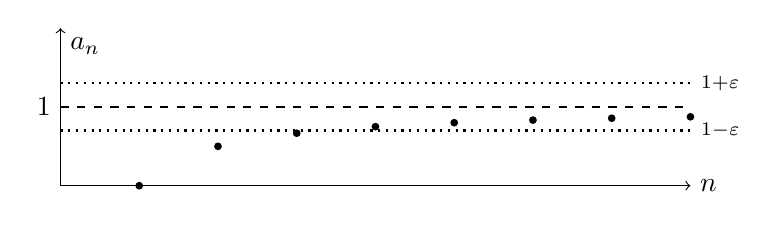
\begin{tikzpicture}
        \def\limitepsilon{0.3}
        \draw[->] (0, 0) -- (0, 2) node[below right] {$a_n$};
        \draw[->] (0, 0) -- (8, 0) node[right] {$n$};
        \draw[dotted, thick] (0, 1 + \limitepsilon) -- (8, 1 + \limitepsilon) node[right] {$\scriptstyle1 + \varepsilon$};
        \draw[dotted, thick] (0, 1 - \limitepsilon) -- (8, 1 - \limitepsilon) node[right] {$\scriptstyle1 - \varepsilon$};
        \draw[dashed] (0, 1) node[left] {1} -- (8, 1);
        \foreach \i in {1, 2, ..., 8} {
          \pgfmathsetmacro{\seq}{1 - 1/\i}
          \fill (\i, \seq) circle (1.4pt);
        }
      \end{tikzpicture}
      \end{center}
      Given $\varepsilon > 0$, using \cref{archimedesCorollary}, choose $N > \frac{1}{\varepsilon}$.
      If $n \geq N$, then:
      \[
        |a_n - 1| = \abs{1 - \frac{1}{n} - 1} = \frac{1}{n} \leq \frac{1}{N} < \varepsilon
      \]
      Hence $a_n \to 1$ as $n \to \infty$.
    \item Consider the sequence $0, \frac{1}{2}, 0, \frac{1}{4}, 0, \ldots$ defined by
      $a_n = \begin{cases}
      \frac{1}{n} & \text{ if $n$ is even} \\
      0 & \text{ if $n$ is odd}
      \end{cases}$
    \begin{center}
    \begin{tikzpicture}
      \def\limitepsilon{0.4}
      \draw[->] (0, -0.7) -- (0, 2) node[below right] {$a_n$};
      \draw[->] (0, 0) node[left] {0} -- (8, 0) node[right] {$n$};
      \draw[dotted, thick] (0, \limitepsilon) -- (8, \limitepsilon) node[right] {$\scriptstyle\varepsilon$};
      \draw[dotted, thick] (0, -\limitepsilon) -- (8, -\limitepsilon) node[right] {$\scriptstyle-\varepsilon$};
      \foreach \i in {1, 2, ..., 8} {
        \ifodd\i
          \pgfmathsetmacro{\seq}{0}
        \else
          \pgfmathsetmacro{\seq}{2/\i}
        \fi
        \fill (\i, \seq) circle (1.4pt);
      }
    \end{tikzpicture}
    \end{center}
    Given $\varepsilon > 0$, pick $N > \frac{1}{\varepsilon}$.
    For the odd terms, we always have $|a_n -0| < \varepsilon$, and for the even terms, if $n \geq N$, then:
    \[
      |a_n - 0| \leq \frac{1}{n} \leq \frac{1}{N} < \varepsilon
    \]
    Hence $a_n \to 0$ as $n \to \infty$
  \item Consider the sequence $\frac{1}{2}, \frac{1}{2} + \frac{1}{4}, \frac{1}{2} + \frac{1}{4} + \frac{1}{8}, \ldots$ defined by $a_n = 1 - \frac{1}{2^{n}}$.
    \begin{center}
    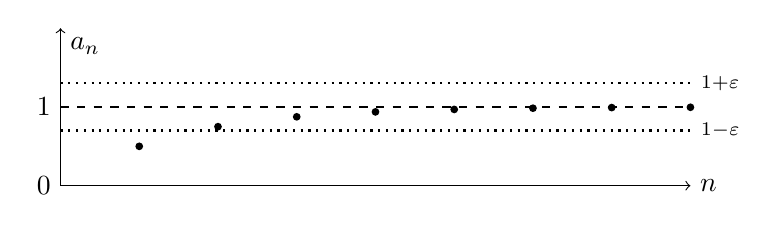
\begin{tikzpicture}
      \def\limitepsilon{0.3}
      \draw[->] (0, 0) -- (0, 2) node[below right] {$a_n$};
      \draw[->] (0, 0) node[left] {0} -- (8, 0) node[right] {$n$};
      \draw[dotted, thick] (0, 1 + \limitepsilon) -- (8, 1 + \limitepsilon) node[right] {$\scriptstyle1 + \varepsilon$};
      \draw[dotted, thick] (0, 1 - \limitepsilon) -- (8, 1 - \limitepsilon) node[right] {$\scriptstyle1 - \varepsilon$};
      \draw[dashed] (0, 1) node[left] {1} -- (8, 1);
      \foreach \i in {1, 2, ..., 8} {
        \pgfmathsetmacro{\seq}{1 - 1/2^\i}
        \fill (\i, \seq) circle (1.4pt);
      }
    \end{tikzpicture}
    \end{center}
    We can see the limit is probably $1$.
    So consider:
    \[
      |a_n - 1| = \frac{1}{2^{n}} \leq \frac{1}{n} \leq \frac{1}{N}
    \]
    Given $\varepsilon > 0$ we would then choose $N > \frac{1}{\varepsilon}$ so that $\frac{1}{N} < \varepsilon$.
    If $n \geq N$ then the above holds true, hence $a_n \to 1$ as $n \to \infty$
  \item $a_n = (-1)^{n}$
      \begin{center}
      \begin{tikzpicture}
        \def\limitepsilon{0.4}
        \draw[->] (0, -1.3) -- (0, 1.3) node[below right] {$a_n$};
        \draw[->] (0, 0) node[left] {0} -- (8, 0) node[right] {$n$};
        \draw[dashed] (0, 0.75) node[left] {1}-- (8, 0.75);
        \draw[dashed] (0, -0.75) node[left] {1}-- (8, -0.75);
        \foreach \i in {1, 2, ..., 8} {
          \pgfmathsetmacro{\seq}{0.75*(-1)^\i}
          \fill (\i, \seq) circle (1.4pt);
        }
      \end{tikzpicture}
      \end{center}
      Let us first show that $a_n \centernot\to 0$.
      We could pick $\varepsilon = 1$ and observe that $|a_n - 0| = 1\ \forall n \in \N$.

      To show that $a_n$ does not converge to any limit (i.e. it diverges), we argue by contradiction.
      Suppose $a_m \to \ell$ as $n \to \infty$ for some $\ell \in \R$.
      Let $\varepsilon = 1$, there must exist some $N \in \N$ such that for all $n \geq N$, $|a_n - \ell| < 1$.
      In particular, $|1 - l| < 1$ and $|-1 - l| < 1$.
      But then
      \[
        2 = |1 - (-1)| = |1 - l + l - (-1)| \leq |1 - l| + |-1 - l| < 2
      \]
      which is a contradiction.
      Hence $((-1)^{n})^{\infty}_{n = 1}$ diverges.
  \end{enumerate}
\end{example}
\begin{remark}[Advice]
  It is difficult to just conjure up a bound on $N$ involving $\varepsilon$.
  Instead, consider the distance between what you think is the limit and $a_n$ and use this to scope out a suitable bound.
\end{remark}
We implicitly assumed that if a limit assumed then it is unique. This can be proven
\begin{proposition}
  If $a_n \to \ell$ as $n \to \infty$, then the limit $\ell$ is unique.
\end{proposition}
\begin{proof}
  Suppose $a_n \to \ell$ and $a_n \to k$ as $n \to \infty$ with $\ell \neq k$.
  Chose $\varepsilon = \frac{1}{2}|\ell - k| > 0$.
  Then $\exists N \in \N$ such that $|a_n - \ell| < \varepsilon$  $\forall n \geq N$ and $\exists M \in \N$ such that $|a_n - k| < \varepsilon$ $\forall n \geq m$.

  But then for any $n \geq \max\{N, M\}$, we have:
  \[
    2\varepsilon = |\ell - k| = |\ell - a_n + a_n - k| \leq |\ell - a_n| + |a_n - k| < 2\varepsilon
  \]
  which is a contradiction.
\end{proof}
\subsection{Boundedness}
\begin{definition}[Bounded Sequence]
  A sequence $(a_n)^{\infty}_{n = 1}$ is \textit{bounded} if there exists a real number $B$ such that
  \[
    |a_n| \leq B,\ \forall n \in \N
  \]
\end{definition}
\begin{remark}
  Any convergent sequence is bounded.
  If $a_n \to \ell$ as $n \to \infty$, then we can take $\varepsilon = 1$ so that $\exists N \in \N$ such that $\forall n \geq N$, $|a_n - \ell| < 1$.
  Hence $|a_n| \leq \max\{|a_1|, |a_2|, \ldots, |a_{N - 1}|, |\ell| + 1\}\ \forall n \in \N$.
\end{remark}
\begin{definition}[Monotonic]
  A sequence $(a_n)^{\infty}_{n = 1}$ is \textit{monotonic} if it is either increasing or decreasing.

  It is \textit{increasing} if $a_{n + 1} \geq a_n\ \forall n \in \N$ and it is \textit{decreasing} if $a_{n + 1} \leq a_n\ \forall \in \N$.
\end{definition}
\begin{theorem}[Monotone Convergence Theorem]
  Every bounded monotonic sequence of real numbers converges.
\end{theorem}
\begin{proof}
  Suppose $(a_n)$ is increasing.
  Then the set $\{a_n: n \geq 1\}$ is a non-empty set which is bounded above as $(a_n)$ is bounded.
  By the least upper bound axiom, it has a supremum, say $\ell$.

  Given $\varepsilon > 0$, $\ell - \varepsilon$ cannot be an upper bound for the set because $\ell$ is the least upper bound.
  Therefore $\exists N \in \N$ such that $a_N > \ell - \varepsilon$.
  Thus, since $(a_n)$ is monotonic $\ell - \varepsilon < a_n \leq \ell$ for $\forall n \geq N$.
  Hence $\forall n \geq N$, $|a_n -\ell| < \varepsilon$ so $a_n \to \ell$.

  The decreasing case is the same but instead considering $(-a_n)$.
\end{proof}
\begin{remark}
  \begin{enumerate}
    \item Note that for an increasing sequence to converge, we only need to use the fact that it is bounded above.
    \item The bounded condition is important. For example, the sequence $(a_n)^{\infty}_{n=1}$ with $a_n = n$ is increasing but not bounded and certainly diverges.
    \item Increasing sequences converge if and only if they are bounded above.
    \item Monotonic Convergence Theorem is in fact equivalent to the least upper bound axiom.
    \item You can in fact show that every sequence has a monotonic subsequence, see Analysis 1.
    \item This does not work over the rational numbers.
      For example, consider the sequence:
      \[
        a_n = \frac{\floor{10^{n}\sqrt{2}}}{10^{n}}
      \]
      That is, $a_n$ gives the first $n + 1$ digits of the decimal expansion of $\sqrt{2}$.
      This is bounded above and increasing sequence of rationals with a limit of $\sqrt{2} \in \R$, but $\sqrt{2} \notin \Q$.
  \end{enumerate}
\end{remark}
\begin{proposition}
  If $a_n \leq d\ \forall n \in \N$ and $a_n \to c$ as $n \to \infty$, then $c \leq d$.
\end{proposition}
\begin{proof}
  Suppose, for contradiction, that $c > d$.
  Let $\varepsilon = c - d > 0$.
  Then $\exists N \in \N$ such that $\forall n \geq N$, $|a_n - c| < \varepsilon$.
  So $|a_n - c| < c - d$.
  Since $a_n \leq d < c$, we have $a_n < c$ so $|a_n - c| = c - a_n$.
  But then we have $c - a_n < c - d \implies a_n > d$ which is a contradiction.
  So we must have $c \leq d$.
\end{proof}
\begin{remark}[Warning]
  If $a_n < d$ $\forall n \in \N$ and $a_n \to c$ as $n \to \infty$ then we need \textbf{not} have $c < d$.

  For example, $\frac{1}{2}, \frac{1}{2} + \frac{1}{4}, \frac{1}{2} + \frac{1}{4} + \frac{1}{8}, \ldots$, whilst each term is less than 1, $\lim_{n \to \infty} a_n = 1$.
\end{remark}
\begin{proposition}
  If $a_n \to c$ as $n \to \infty$ and $b_n \to d$ as $n \to \infty$, then $a_n + b_n \to c + d$ as $n \to \infty$
\end{proposition}
\begin{proof}
  Given $\varepsilon > 0$, $\exists N \in \N$ such that $\forall n \geq N, |a_n - c| < \frac{\varepsilon}{2}$, and $\exists M \in \N$ such that $\forall n \geq M, |b_n - d| < \frac{\varepsilon}{2}$.

  If we choose $N' = \max\{N, M\}$, then $\forall n \geq N'$:
  \[
    |a_n + b_n - (c + d)| \leq |a_m - c| + |b_n - d| < \frac{\varepsilon}{2} + \frac{\varepsilon}{2} = \varepsilon
  \]
  So $a_n + b_n \to c + d$.
\end{proof}
\begin{remark}[Note]
  When doing a proof like this, it is \textbf{not} imperative that you end up with just $< \varepsilon$ at the end.
  In the above proof it would be fine to have ended up with $2\varepsilon$ as we could just make the original $\varepsilon$ smaller.
\end{remark}
\end{document}
